\subsection{Test setup}

Our program was written in C/C++ and compiled with Clang. All memory allocations were cache line boundary aligned. For parallelization we used C++11 cross-platform library \texttt{<thread>}.

All benchmarks were performed on a Linux desktop which has 4 GB ram and a Core i3 550 CPU with the following specification:

\begin{itemize}
\item 2 * 3.2 GHz (no Turbo boost)
\item 2 * 32 KB L1 instruction cache
\item 2 * 32 KB L1 data cache
\item 2 * 256 KB L2 cache
\item Shared 4 MB L3 cache
\item 64 byte cache lines
\item Inclusive caches
\item The associativity for the cache levels are 8, 8 and 16 respectively
% http://www.ni.com/white-paper/11266/en#toc5
\end{itemize}

L2 cache faults and L3 cache faults were measured using Intel Performance Monitor Counter while branch mispredictions were measured using PAPI.

All tests were performed 5 times and the median was selected. The data in the matrices were randomly generated double precision floating points with
an uniform distribution. The range of the data was 0 to
10,000.

\subsection{Simple multiplication}

\subsubsection{Row-based layout}

\ref{fig:rnrnrn0}

\begin{figure}[h!]
  \centering
  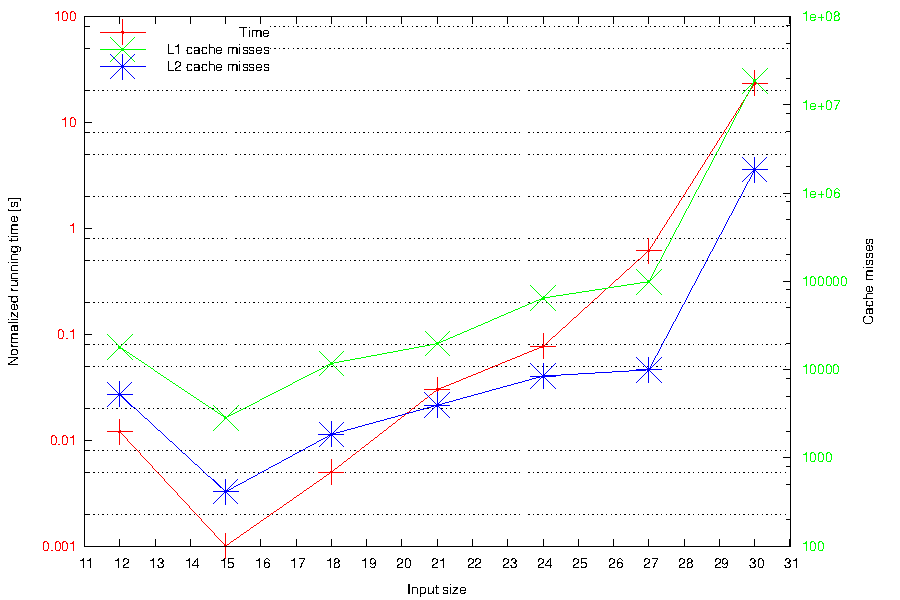
\includegraphics[width=\textwidth]{rnrnrn0.pdf}
  \label{fig:rnrnrn0}
\end{figure}

\subsubsection{Combined row-based and column-based layout}

\ref{fig:rncnrn0}

\begin{figure}[h!]
  \centering
  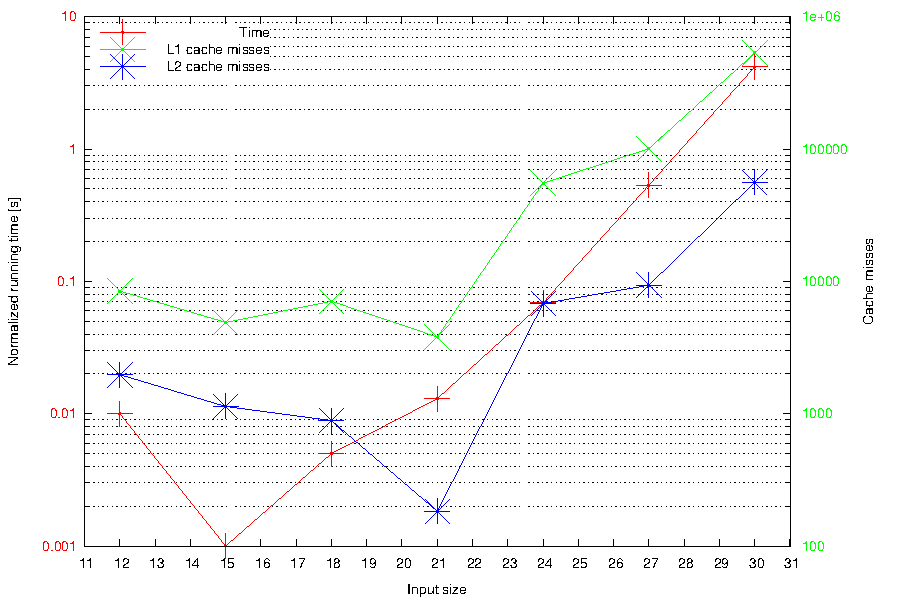
\includegraphics[width=\textwidth]{rncnrn0.pdf}
  \label{fig:rncnrn0}
\end{figure}

\subsection{Recursive multiplication}

\subsubsection{Z-curve layout}

\ref{fig:zrzrzr0}

\begin{figure}[h!]
  \centering
  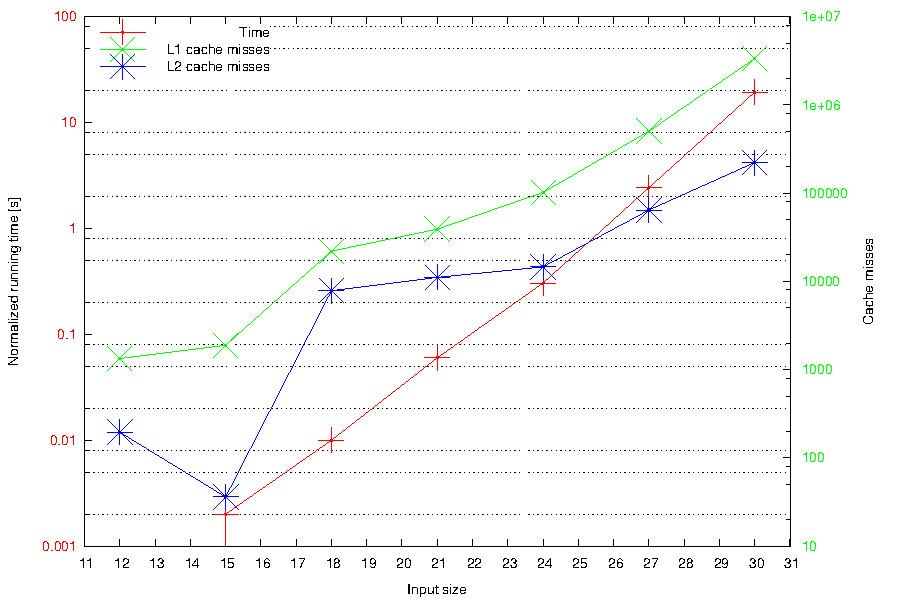
\includegraphics[width=\textwidth]{zrzrzr0.pdf}
  \label{fig:zrzrzr0}
\end{figure}